%%%%%%%%%%%%%%%%%%%%%%%%%%%%%%%%%%%%%%%%%
% a0poster Portrait Poster
% LaTeX Template
% Version 1.0 (22/06/13)
%
% The a0poster class was created by:
% Gerlinde Kettl and Matthias Weiser (tex@kettl.de)
% 
% This template has been downloaded from:
% http://www.LaTeXTemplates.com
%
% License:
% CC BY-NC-SA 3.0 (http://creativecommons.org/licenses/by-nc-sa/3.0/)
%
%%%%%%%%%%%%%%%%%%%%%%%%%%%%%%%%%%%%%%%%%

%----------------------------------------------------------------------------------------
%	PACKAGES AND OTHER DOCUMENT CONFIGURATIONS
%----------------------------------------------------------------------------------------

\documentclass[a0,portrait]{a0poster}
\usepackage[utf8]{inputenc}
\usepackage[francais]{babel}
\usepackage[T1]{fontenc}

\usepackage{multicol} % This is so we can have multiple columns of text side-by-side
\columnsep=100pt % This is the amount of white space between the columns in the poster
\columnseprule=3pt % This is the thickness of the black line between the columns in the poster

\usepackage[svgnames]{xcolor} % Specify colors by their 'svgnames', for a full list of all colors available see here: http://www.latextemplates.com/svgnames-colors

\usepackage{times} % Use the times font

\usepackage{graphicx} 
\usepackage{booktabs} % Top and bottom rules for table
\usepackage[font=large,labelfont=bf]{caption} % Required for specifying captions to tables and figures
\usepackage{amsfonts, amsmath, amsthm, amssymb} 
\usepackage{wrapfig} % Allows wrapping text around tables and figures
\usepackage{tikz}
% \usetikzlibrary{calc,trees,positioning,arrows,chains,shapes.geometric,%
% decorations.pathreplacing,decorations.pathmorphing,shapes,%
% matrix,shapes.symbols,plotmarks,decorations.markings,shadows}
\usepackage[most]{tcolorbox}
\usepackage{array}

\newcommand{\captioncolor}{\color{black}}

\begin{document}
\large
%----------------------------------------------------------------------------------------
%	POSTER HEADER 
%----------------------------------------------------------------------------------------

% The header is divided into two boxes:
% The first is 75% wide and houses the title, subtitle, names, university/organization and contact information
% The second is 25% wide and houses a logo for your university/organization or a photo of you
% The widths of these boxes can be easily edited to accommodate your content as you see fit

\begin{minipage}[b]{0.8\linewidth}
\veryHuge \color{NavyBlue} \textbf{Stage de Recherche en Informatique (Sup\'e{}lec 2A)} \color{Black}\\ 
\Huge\textit{ Génération de signaux micro-Doppler par réseaux de neurone }\\[18mm]
\huge \textbf{Paul LE GRAND DES CLOIZEAUX}\\[0.5cm] 
\huge LRI, CentraleSupélec, Université Paris-Saclay\\[0.4cm] 
\end{minipage}
%
\begin{minipage}[b]{0.25\linewidth}

\includegraphics[width=15cm]{logo_lri.jpg}\\
\end{minipage}

\vspace{1cm} % A bit of extra whitespace between the header and poster content

%----------------------------------------------------------------------------------------

\begin{multicols}{2} % This is how many columns your poster will be broken into, a portrait poster is generally split into 2 columns

%----------------------------------------------------------------------------------------
%	CONTEXTE
%----------------------------------------------------------------------------------------

% \begin{tcolorbox}[colback=blue!5!white,colframe=blue!75!black,title={\section*{Contexte du stage}}]

% Ce stage a été réalisé cet été (stage de 2A) au Laboratoire de Recherche en Informatique, sous la direction du Pr. Joanna Tomasik. Si la plupart des stages se font en entreprise, j'ai préféré effectuer un stage de recherche, continuant mon apprentissage en recherche initié lors du projet long. J'ai travaillé pendant deux mois avec Julien Gérard, doctorant, sur un des problèmes qu'il traite dans sa thèse.

% \end{tcolorbox}

\begin{tcolorbox}[colback=blue!5!lime,colframe=green!75!black,title={\section*{Contexte}}]
\textbf{Objectif: Classifier des profils micro-Doppler d'objets volants}\\
Des profils micro-Doppler de drones et d'oiseaux ont été collectés par l'ONERA.\\
\end{tcolorbox}


%----------------------------------------------------------------------------------------
%	Profils micro-Doppler
%----------------------------------------------------------------------------------------

\begin{tcolorbox}[colback=blue!5!white,colframe=blue!75!black,title={\section*{Profils micro-Doppler}}]
\textbf{Format: Spectrogramme en temps long}
\begin{center}
    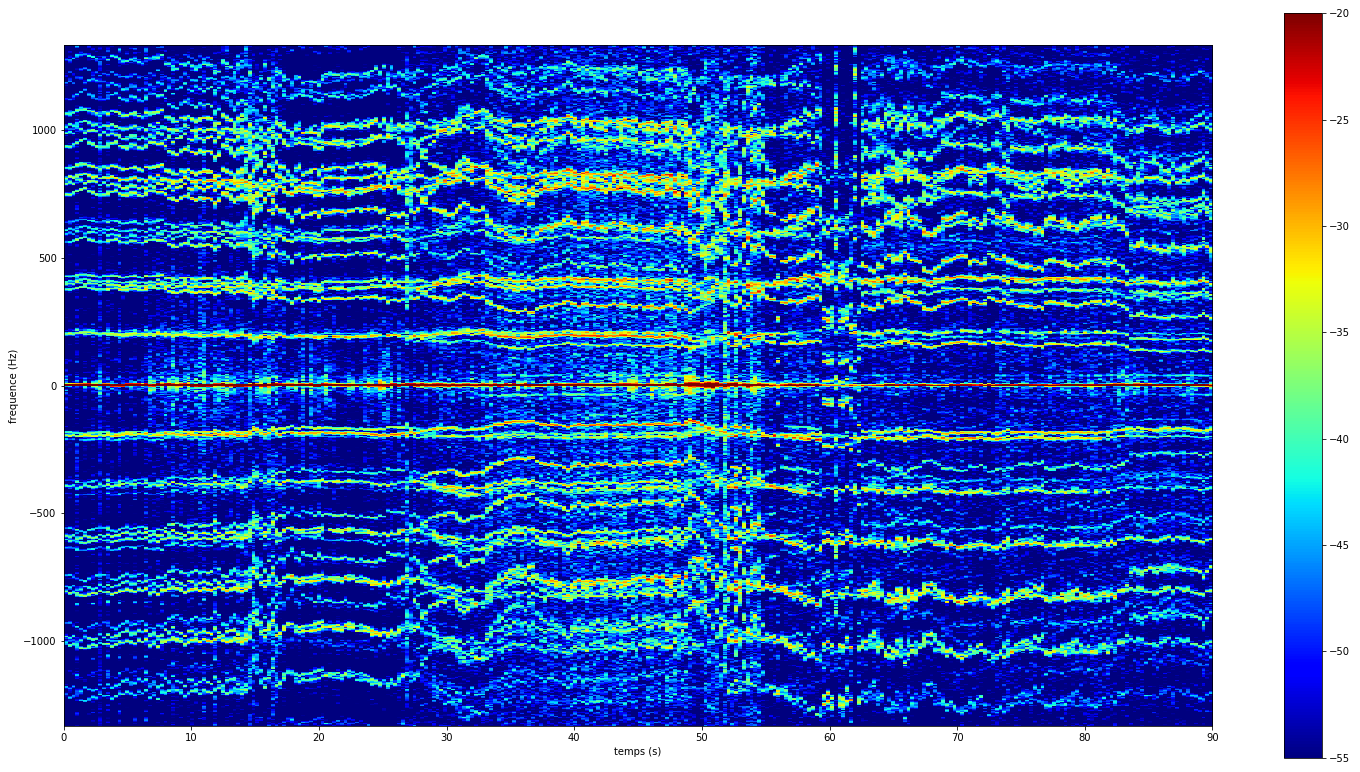
\includegraphics[width=0.8\textwidth]{./QD41_2.png}
    \captionof{figure}{\captioncolor Spectrogramme en temps long d'un drone}
    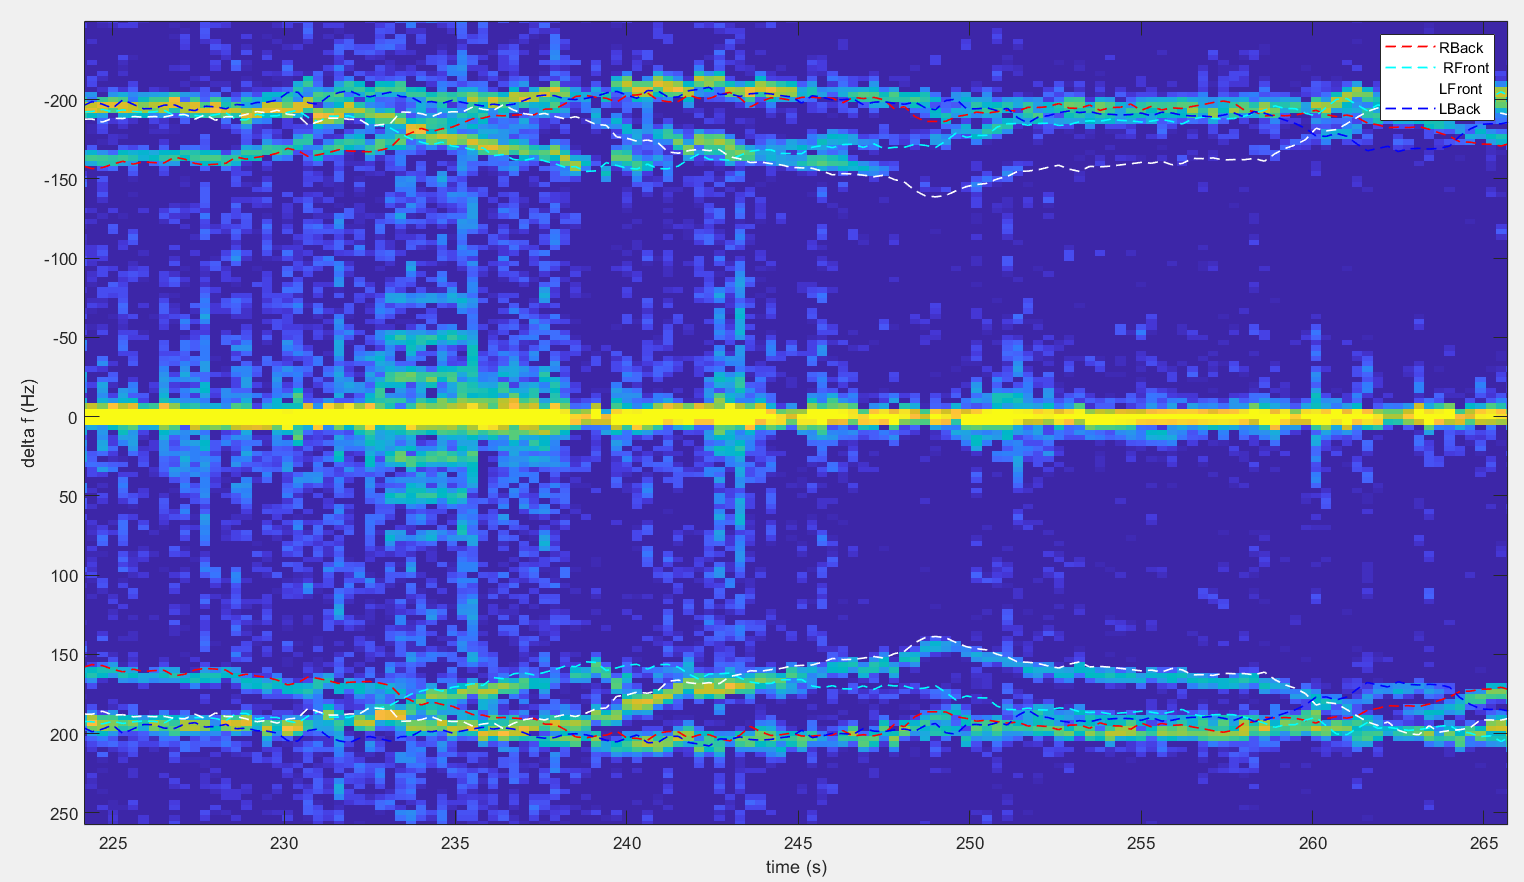
\includegraphics[width=0.8\textwidth]{./QD41_close.png}
    \captionof{figure}{\captioncolor Zoom - décalages de fréquences dus aux rotors}
\end{center}
\end{tcolorbox}

%----------------------------------------------------------------------------------------
%	Qu'est ce qu'un GAN?
%----------------------------------------------------------------------------------------
\begin{tcolorbox}[colback=blue!5!white,colframe=blue!75!black,title={\section*{Quantité de donnés insuffisantes}}]

\textbf{Problèmes}\\
\begin{itemize}
    \item Nombre faible de profils.
    \item Profils hautement corrélés (collectés dans des conditions semblables)
\end{itemize}
\textbf{Solution proposée}\\
Génération de profils micro-Doppler artificiels par réseaux de neurone (\textbf{GAN}).\\
\end{tcolorbox}

%----------------------------------------------------------------------------------------
%	Qu'est ce qu'un GAN?
%----------------------------------------------------------------------------------------

\begin{tcolorbox}[colback=blue!5!white,colframe=blue!75!black,title={\section*{Qu'est ce qu'un GAN (Generative Adversarial Network)?}}]
\begin{center}
    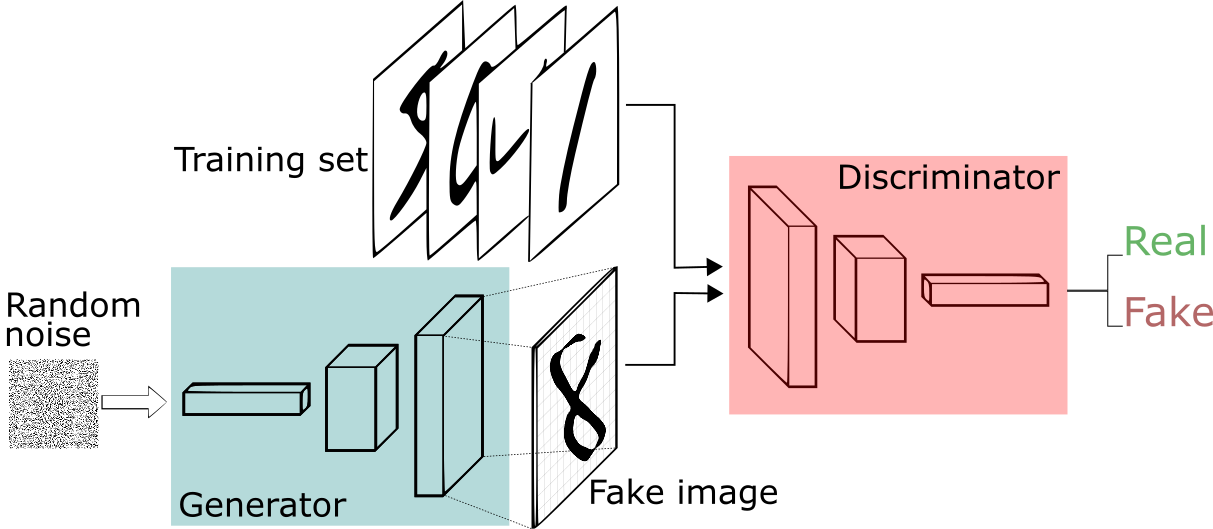
\includegraphics[width=0.9\textwidth]{./gan_schema}
    \captionof{figure}{\captioncolor Schéma d'un GAN basique} 
\end{center}
Un GAN : un réseau de neurone utilisé pour générer des données de manière non-supervisé.

\subsection*{Fonctionnement}
Équilibre entre le \textbf{generateur} et le \textbf{discriminateur}
\end{tcolorbox}

%----------------------------------------------------------------------------------------
%	Comment mesurer les performances d'un GAN?
%----------------------------------------------------------------------------------------

\begin{tcolorbox}[colback=blue!5!lime,colframe=green!75!black,title={\section*{Comment mesurer les performances d'un GAN?}}]
Contrairement à un modèle de classification ou de régression supervisé, pas de possibilité de comparer à une base de test\\

On voudrait pouvoir comparer et quantifier une "distance" entre la distribution des images générés et la distribution des images réels.

\end{tcolorbox}

%----------------------------------------------------------------------------------------
%	FID
%----------------------------------------------------------------------------------------

\begin{tcolorbox}[colback=blue!5!white,colframe=blue!75!black,title={\section*{FID}}]
 
Pour cela on utilise \textbf{InceptionV3}, un réseau de neurone à convolution, pour faire un \textit{embedding}
des images en un vecteur de taille 2048.\\
On récupère la valeur de la dernière couche d'InceptionV3 pour chacun des éléments générés.

\begin{center}
    $$X_{\mbox{\small real}}=\mathcal{N}(\mu_{real}, \Sigma_{real}), X_{generated}=\mathcal{N}(\mu_{generated}, \Sigma_{generated})\\
    FI = ||\mu_{real} - \mu_{generated}|| $$
\end{center}

\end{tcolorbox}

%----------------------------------------------------------------------------------------
%	Résultats
%----------------------------------------------------------------------------------------

\begin{tcolorbox}[colback=blue!5!white,colframe=blue!75!black,title,title={\section*{Résultats}}]
\end{tcolorbox}


%----------------------------------------------------------------------------------------
%	PERSPECTIVES
%----------------------------------------------------------------------------------------

\begin{tcolorbox}[colback=red!5!orange,colframe=red!75!black,title={\section*{Perspectives}}]
\end{tcolorbox}
\end{multicols}
\end{document}
